\chapter{Normalization of metadata in the Sequence Read Archive} \label{chap:1}

The work in this chapter was previously published as \textit{MetaSRA: normalized human sample-specific metadata for the Sequence Read Archive} (\citealp{Bernstein2017}). 

\section{Background}

The SRA promises great biological insight if one could analyze the data in the aggregate; however, the data remain largely underutilized, in part, due to the poor structure of the metadata associated with each sample. The rules governing submissions to the SRA do not dictate a standardized set of terms that should be used to describe the biological samples from which the sequencing data are derived. As a result, the metadata include many synonyms, spelling variants and references to outside sources of information. Furthermore, manual annotation of the data remains intractable due to the large number of samples in the archive. For these reasons, it has been difficult to perform large-scale analyses that study the relationships between biomolecular processes and phenotype across diverse diseases, tissues and cell types present in the SRA.

Our goal in this work is to provide structured descriptions of the human biological samples used in the SRA in order to enable aggregate analysis, as well as reanalysis, of these data.  This task is challenging because it requires discriminating between information that describes the biological sample from information that describes other entities such as the sample's study, sequencing protocol, and lab. A solution to structuring the sample-specific information must address the metadata's semantics. 

Existing methods for normalizing biomedical text focus on annotating the text with terms in a controlled vocabulary, usually in the form of a biomedical ontology.  One can approach the task of annotating metadata using either a manual or automated approach.  Manual annotation allows for high accuracy at the cost of low throughput.  For example, the RNASeqMetaDB  provides a database of manually annotated terms associated with a set of mouse RNA-seq experiments (\citealp{Guo}).  This database describes only 306 RNA-seq experiments, which represents a small subset of all experiments in the SRA. 

In contrast, automated annotation allows higher throughput at the cost of lower accuracy. Methods for automating the normalization of biomedical metadata frame the task as that of \textit{entity recognition}. Entity recognition is the process of automatically recognizing and linking entities in natural language text to their corresponding entries in a controlled vocabulary.  Tools that take this approach include ConceptMapper (\citealp{Tanenblatt}), SORTA (\citealp{Pang}), ZOOMA (\citealp{Misha}), and the BioPortal Annotator (\citealp{Noy}).  Furthermore, there have been efforts to utilize such tools to automatically normalize large biomedical metadata sets.  For example, work by \cite{Shah} automatically annotated samples and studies in the Gene Expression Omnibus (GEO) (\citealp{Barrett2013}) and other sources of biomedical metadata. Similarly, work by \cite{Galeota} annotated samples in GEO using ConceptMapper. 

We assert that entity recognition alone is insufficient for automating the normalization of the SRA's sample-specific metadata.  Rather, since many of the sample's descriptions mention ontology terms that describe extraneous entities (such as the study and experiment), a suitable solution should seek to extract \textit{only} those terms that are being used to describe the biology of the sample. Biomedical entity recognition tools are best suited for data submitters who wish to facilitate annotation of their metadata before submission. Such tools do not adequately filter terms that do not describe the biology of the sample because they do not attempt to understand the fine-grained semantics of the text.

We further assert that important biological properties are often numerical and are not captured by ontology terms alone.  Such terms include age, time point, and passage number for cell cultures. To the best of our knowledge, the problem of extracting real-value properties from metadata has yet to be addressed.

Lastly, we assert that ontology terms alone do not always provide enough context to understand the type of sample being described.  For example, a cell culture that consists of stem cells differentiated into fibroblast cells may be annotated as both ``stem cells'' and as ``fibroblast.''  Such annotation leaves ambiguity as to whether the sample was differentiated from stem cells, or rather, was reprogrammed into a pluripotent state from primary fibroblasts.  We assert that each sample should be categorized into a specific sample-type that captures the process that was used to obtain the sample.  

To address problems in the SRA's metadata, we developed MetaSRA: a normalized encoding of biological samples in the SRA, along with the novel computational pipeline with which it was automatically constructed.   MetaSRA encodes the metadata for each sample with a schema inspired by that used in the ENCODE project (\citealp{Malladi}).  This schema is comprised of three parts:
\begin{enumerate}
\item Sample labels, using terms from the following biomedical ontologies: Disease Ontology (\citealp{Kibbe}), Cell Ontology (\citealp{Bard}), Uberon (\citealp{Mungall}), Experimental Factor Ontology (EFO) (\citealp{Malone}), and the Cellosaurus (\citealp{Bairoch2018}). 
\item A sample-type classification, with six sample-type categories similar to those used by ENCODE.
\item Standardized numerical properties of the sample.
\end{enumerate}
The first two parts are shared with the ENCODE schema, with the last part being a MetaSRA-specific extension. Currently, MetaSRA encodes all human samples utilized in RNA-seq experiments on the Illumina platform; however, future work will expand MetaSRA to other species and assays.

\begin{figure*}[!tpb]
\centerline{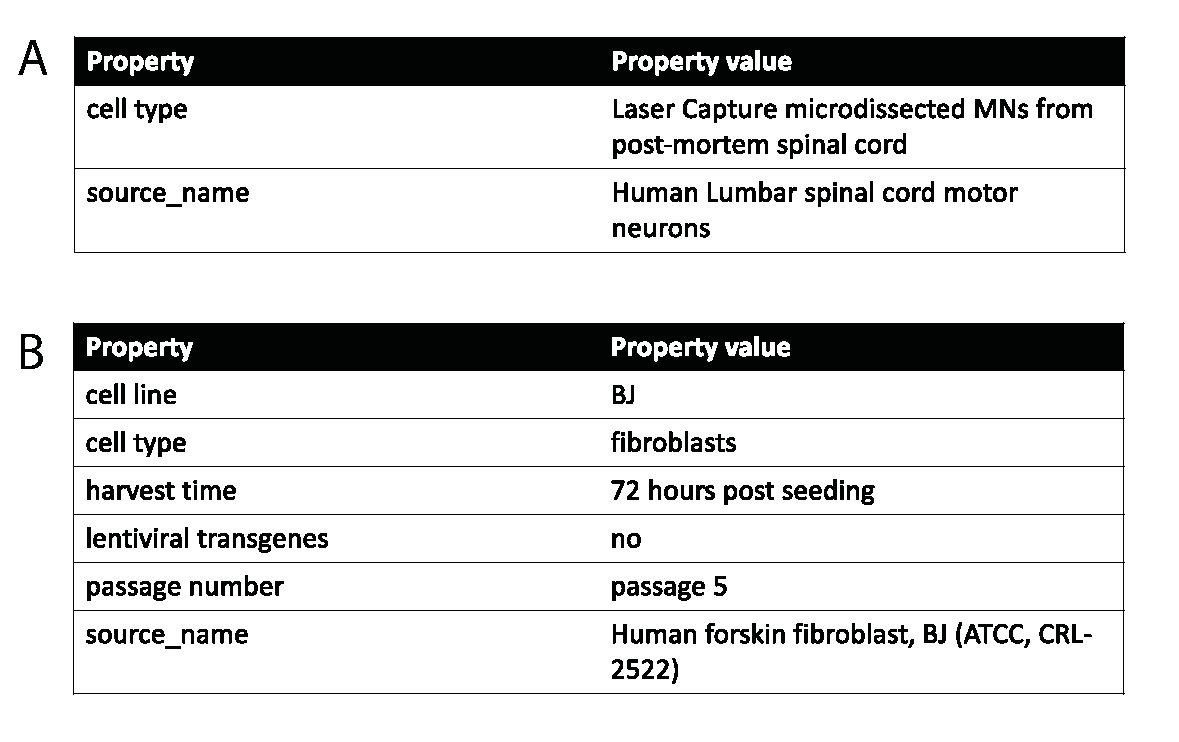
\includegraphics[width=13cm]{figures/example_key_vals.eps}}
\caption{\textbf{Example metadata entries.} (A) Sample-specific key-value pairs describing sample SRS1217219. Note that the values encode natural language text. (B) Sample-specific key-value pairs describing sample SRS872370. Note the reference to an external cell lin
e BJ. We also note that `forskin fibroblast' is an incorrect spelling. Lastly, the value `no' negates the key `lentiviral transgenes.'}
\label{fig:example_raw_key_vals}
\end{figure*}

\section{Task definition}

\subsection{Mapping samples to ontologies}

Like the ENCODE project, we label each biological sample using biomedical ontologies. We define the task of mapping samples to ontologies as follows: given a set of samples $\mathcal{S}$, a set of ontology terms $\mathcal{O}$, and set of relationship-types $\mathcal{R}$, we seek a function $f: \mathcal{S} \rightarrow \mathscr{P}(\mathcal{O})$, where $\mathscr{P}(\mathcal{O})$ is the powerset of $\mathcal{O}$, such that given a sample $s$, for each $o \in f(s)$, there exists a relationship-type $r \in \mathcal{R}$ that relates the sample $s$ to the ontology term $o$.   We restrict $\mathcal{R}$ to the following types of relationships:
\begin{itemize}
    \item \textbf{has phenotype}:  Maps samples to phenotypic or disease terms. 
    \item \textbf{derives from}:   Maps samples to cell lines or, when the sample consists of differentiated cells, to stem cell terms. 
    \item \textbf{part of}:    Maps samples to the anatomical entity from which it was extracted. 
    \item \textbf{consists of cells of type}:  Maps samples to their constituent cell types. 
    \item \textbf{underwent}: Maps samples to ontology terms that describe a medical or experimental protocol. \vspace*{1pt}
\end{itemize}
We restrict our use of ontology terms to only ``biologically significant'' terms.  An ontology term $o$ is deemed biologically significant if given two samples $s_1, s_2 \in \mathcal{S}$  where $f(s_1) \subset f(s_2)$ and $f(s_2) \setminus f(s_1) = \{o\}$
 there likely exists a difference in gene expression or other measurable difference in biochemistry between the two samples.  In simpler terms, an ontology term $o$ is deemed biologically significant if given two samples with equivalent descriptions barring that one sample can be described by $o$ and the other cannot, a significant difference in the biochemistry of the cell may exist between the two samples. For example, the ontology term for ``cancer'' is biologically significant, whereas the term ``organism'' is not because all samples are trivially derived from an organism.   We manually searched the ontologies for biologically significant terms that are near the roots of the ontologies' directed acyclic graphs.  We then assume that all children of a biologically significant term are also biologically significant and retrieve all children of the manually selected nodes. We map samples to only biologically significant terms in the ontologies.  An example of a standardized sample is shown in Figure~\ref{fig:project_flow}.
 
 \subsubsection{Discriminating between term mentions and term mappings}

Our goal in mapping samples to ontology terms goes beyond named entity recognition.  Rather than finding all occurrences or ``mentions'' of ontology terms in the metadata, we attempt to infer which labels adequately describe the biological sample being described.  A term may be mentioned, but not mapped as well as mapped, but not mentioned. 

For example, consider a sample's description that includes the following text: \texttt{Metastatic castration resistant}\\ \texttt{prostate cancer}.  If we consider the Uberon and Disease Ontology, we see that the string ``prostate cancer'' mentions three terms in these ontologies: ``prostate gland'', ``cancer'', and ``prostate cancer.'' Of these terms, only ``cancer'' and ``prostate cancer'' are mapped because they are related to the sample through the ``has phenotype'' relationship. The string ``prostate'' is not not mapped because it localizes the disease rather than the sample.  There is no relationship-type in $\mathcal{R}$ that associates the sample with ``prostate.''  By prohibiting the mapping to ``prostate'', we remove ambiguity as to whether the sample was derived from an organism with a prostate-related disease, or from prostate tissue itself.  More generally, whenever a sample maps to an anatomical entity, we are asserting that the sample originated from that site.

To provide an example in which an ontology term should be mapped, but is not mentioned, consider a sample described with the key-value pair \texttt{passage: 4}.  The Cell Ontology term for ``cultured cell'' is not mentioned in this description; however, by the fact that it was explicitly stated that the cell was passaged, we can infer that the sample consists of cultured cells. Thus we map the sample to ``cultured cell'' via the ``consists of cells of type'' relationship.

\subsubsection{Discriminating between explicit and consequent mappings}

We distinguish between two types of mappings: those that are explicit in the metadata and those that can be inferred from the explicit mappings.   We refer to the latter as ``consequent mappings.''  For example, the ontology term for ``female'' is explicitly mapped from the key-value pair, \texttt{sex: female}, because the author is explicitly communicating the fact that this sample maps to ``female'' through the ``has phenotype'' relationship.

A sample ``consequently'' maps to an ontology term if, using external knowledge, one can logically conclude that the sample maps to the term. The premier example of such a case arises when a sample maps to a cell line.  In such a case, the sample would consequently map to terms that describe this cell line. For example, given the key-value pair \texttt{cell line: MCF-7}, the sample would consequently map to ``adenocarcinoma'' because the MCF-7 cell line was established from a breast adenocarcinoma tumor.  MetaSRA includes both explicit and consequent mappings.

\subsection{Extracting real-value properties}
In addition to mapping samples to ontology terms, we also annotate samples with real-value properties that are described in the metadata.  We structure each real-value property as a triple ($property$, $value$, $unit$) where $property$ is a property ontology term in the EFO, $value \in \mathbb{R}$, and $unit$ is an ontology term in the Unit Ontology (\citealp{Gkoutos}).  For example, the raw key-value pair \text{\texttt{age: 20 years old}} would map to the tuple (``age'', 20, ``year'').

\subsection{Predicting sample-type category}

Like the ENCODE project, we categorize samples into their respective sample-type using categories similar to those used by ENCODE.  These categories consist of \texttt{cell line}, \texttt{tissue}, \texttt{primary cell}, \texttt{stem cell}, \texttt{in vitro differentiated cells}, and \texttt{induced pluripotent stem cell line}. Whereas ENCODE uses an \texttt{immortalized cell line} category, we instead use the category \texttt{cell line} to generalize to any cells that have been passaged multiple times, which include those from finite cell lines.  Figure~\ref{fig:sample_type_def} illustrates how we define each sample-type category based on the methods by which the sample was obtained. We note that we call an isolated cell sample a ``stem cell" if the targeted cell type has the ability to differentiate.  Thus, the ``stem cell" category includes any cell type that is pluripotent, multipotent, or oligopotent.   

\begin{figure}[htbp]
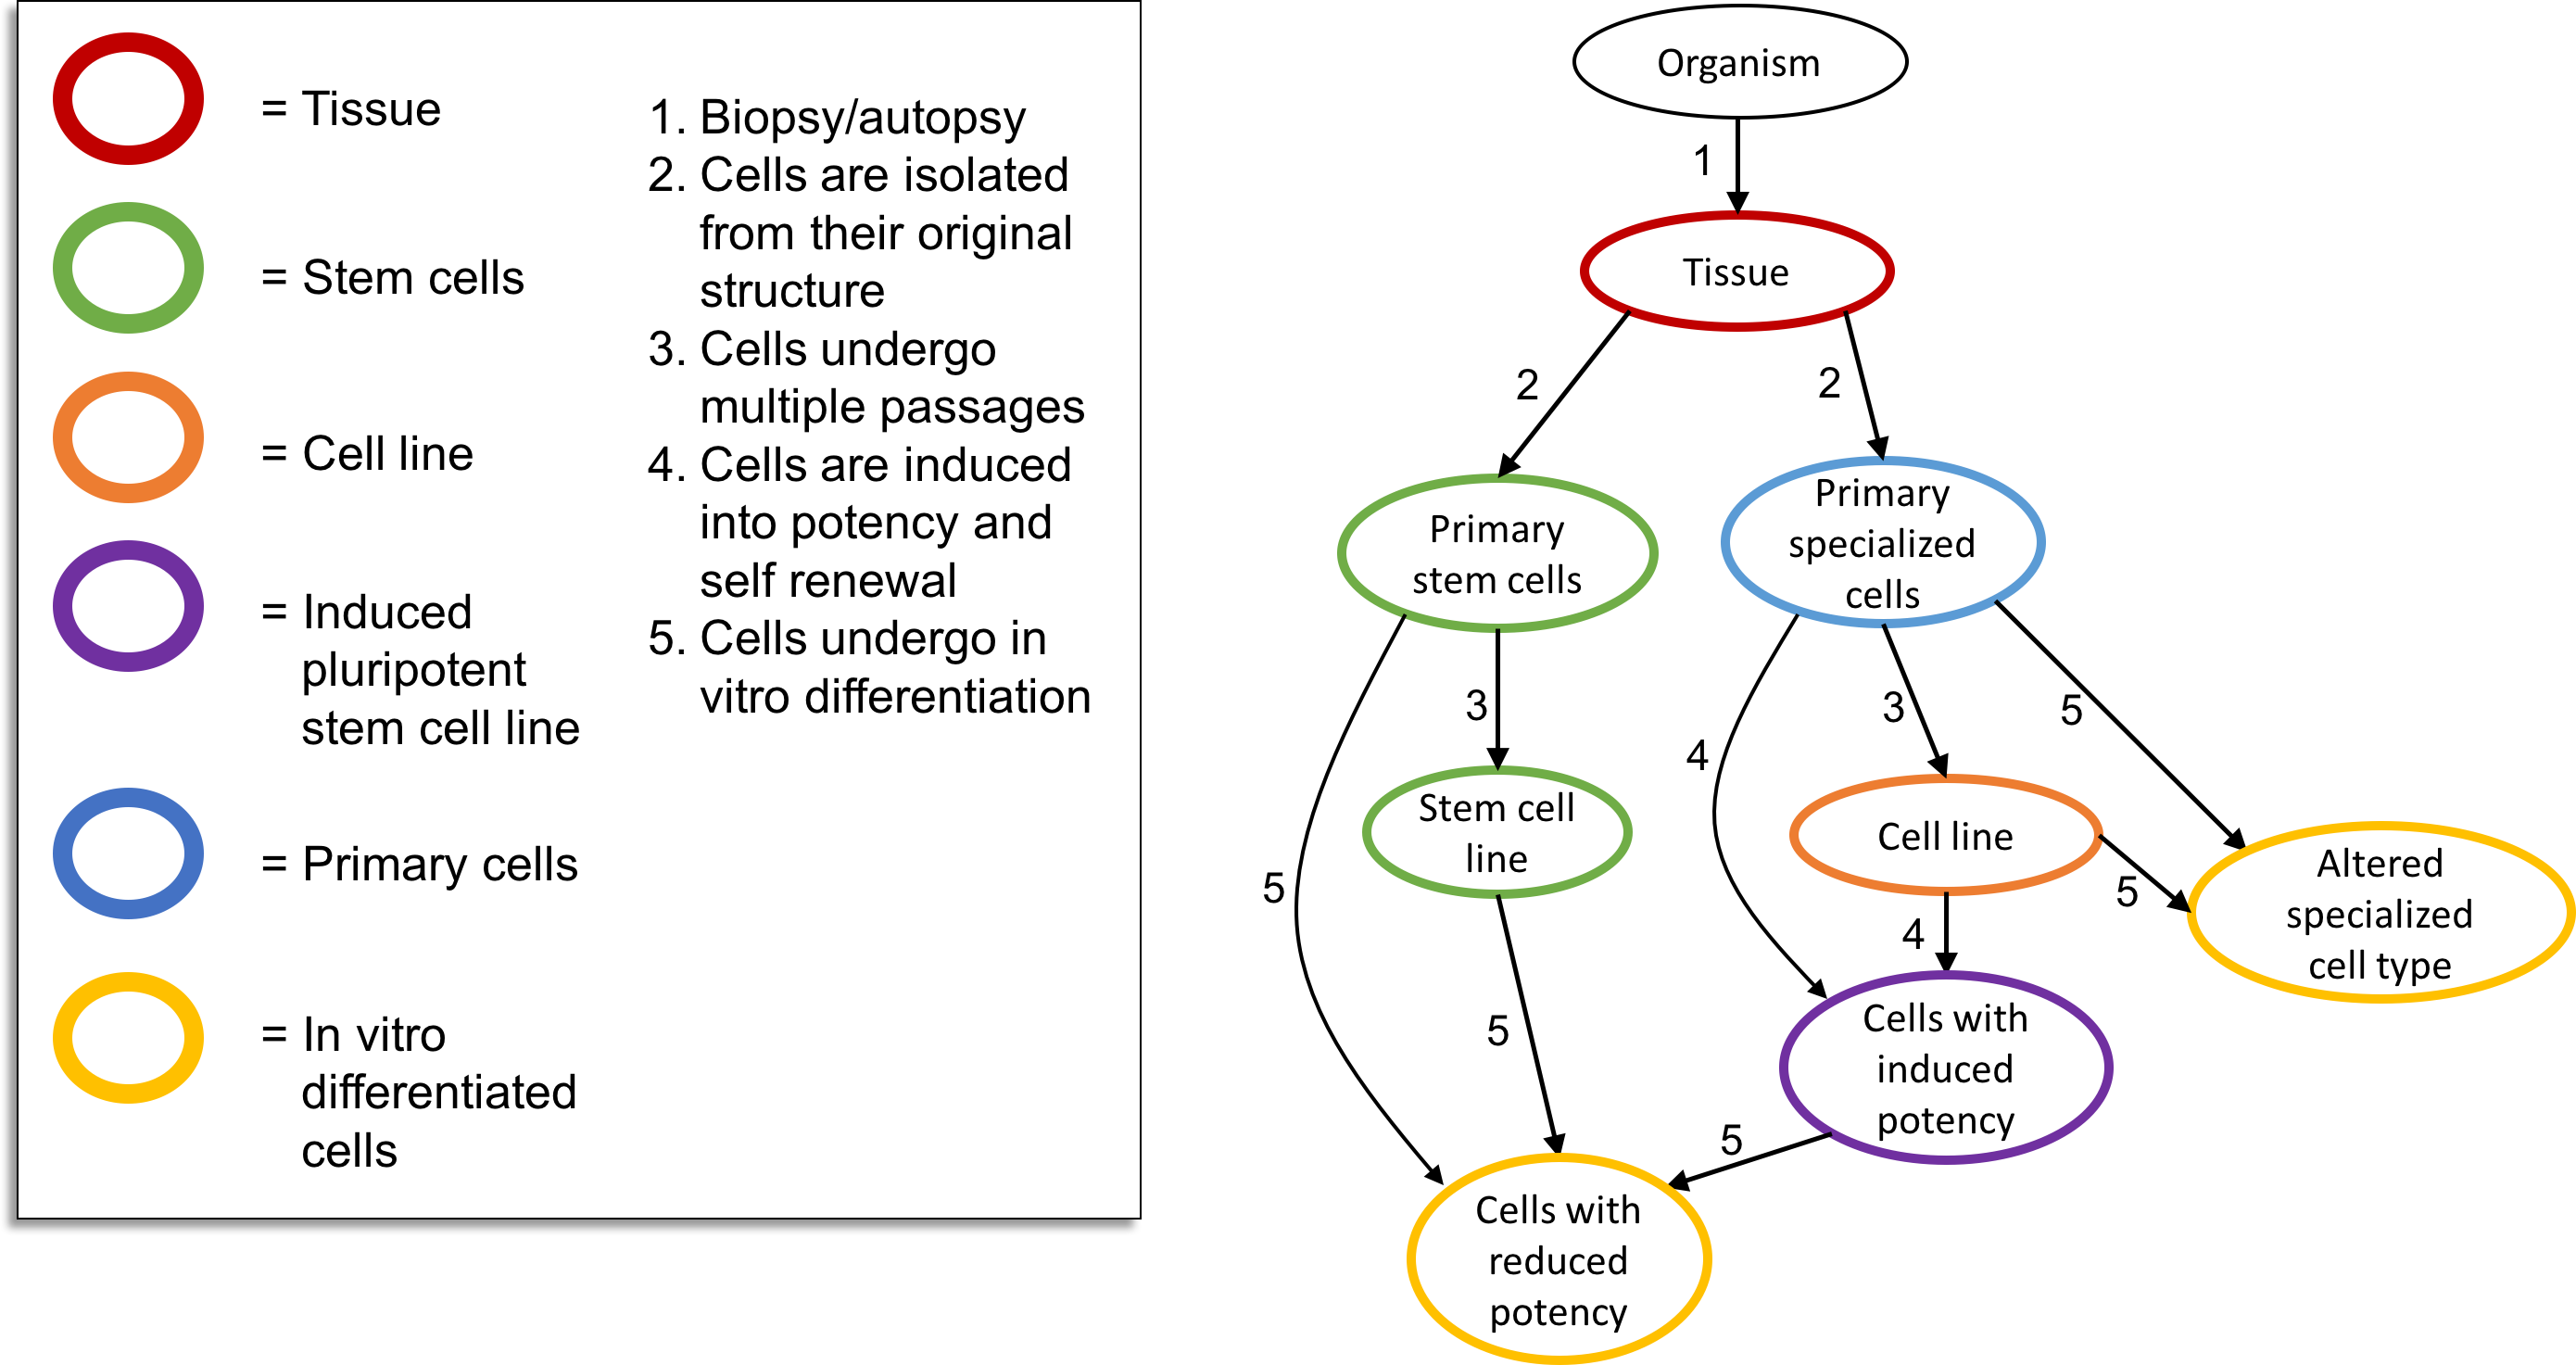
\includegraphics[width=13cm]{figures/sample_type_definition.png}  
\caption{\textbf{Sample-type definitions.} A graph illustrating how sample-type categories are defined. Each node in the graph represents a biological sample.  Arrows between nodes represent procedures carried out on the sample.  Nodes are colored according to their sample-type category.}
\label{fig:sample_type_def}
\end{figure}





\section{Data}

\begin{figure*}[!tpb]
\centerline{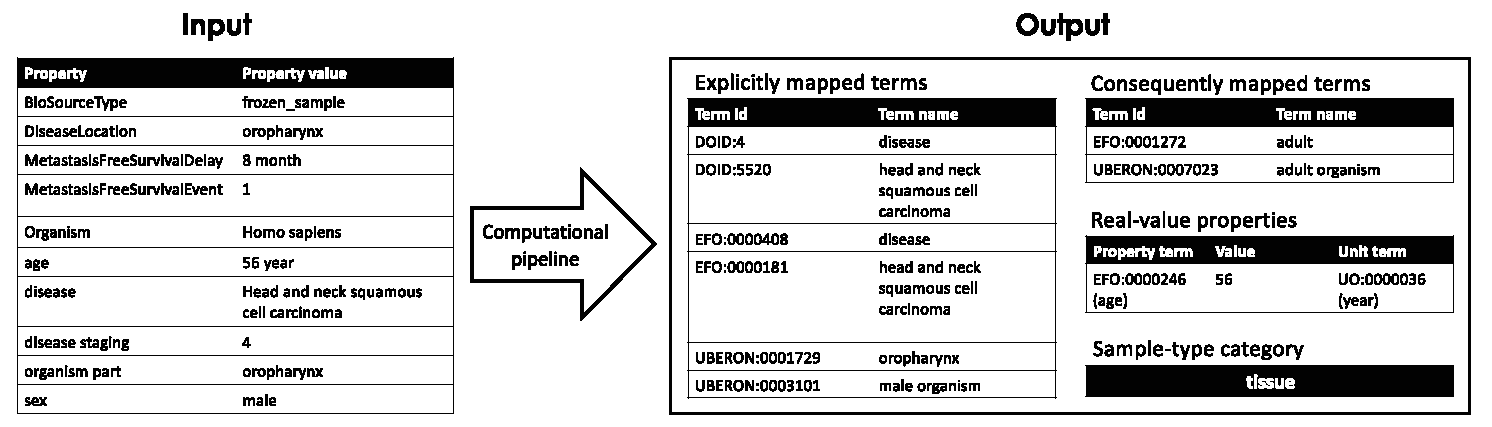
\includegraphics[width=13cm]{figures/project_flow.pdf}}
\caption{\textbf{Example of metadata normalization.} An example of the metadata normalization process for sample ERS183215. We extract explicit mappings, consequent mappings, real-value properties, and the sample-type category for each set of sample-specific key-value pairs in the SRA.}
\label{fig:project_flow}
\end{figure*}

We standardized all human samples assayed by RNA-seq experiments on the Illumina platform.  Metadata was retrieved from the SRAdb (\citealp{Yuelin}) downloaded on 09/05/2016.  The BioSample's sample-specific key-value pairs are  stored in the ``attribute'' field of the ``sample'' table in the SRAdb.  Our data set consists of 75,038 samples, of which, 73,407 are associated with a non-empty set of descriptive key-value pairs.

The samples processed belong to 2,681 distinct studies and the number of samples contained in each study varies by several orders of magnitude (Fig.~\ref{fig:dataset}C).  These studies can be partitioned into 88 ``large" ($\geq 100$ samples) and 2,593 ``small'' ($< 100$ samples) studies, with the ``large'' studies constituting 57\% of all samples processed.  Due to the fact that samples belonging to a common study are described similarly, we argue that it is tractable to annotate samples belonging to the modest number of ``large'' studies using hand-tuned study-specific methods.  In contrast, the large number of ``small'' studies and the diversity of their associated descriptions makes the process of designing study-specific methods for all of these studies intractable.  We therefore focused our evaluations on samples belonging to ``small'' studies, with future work involving hand-tuning the normalization of samples from ``large'' studies.

\begin{figure*}[!tpb]
\centerline{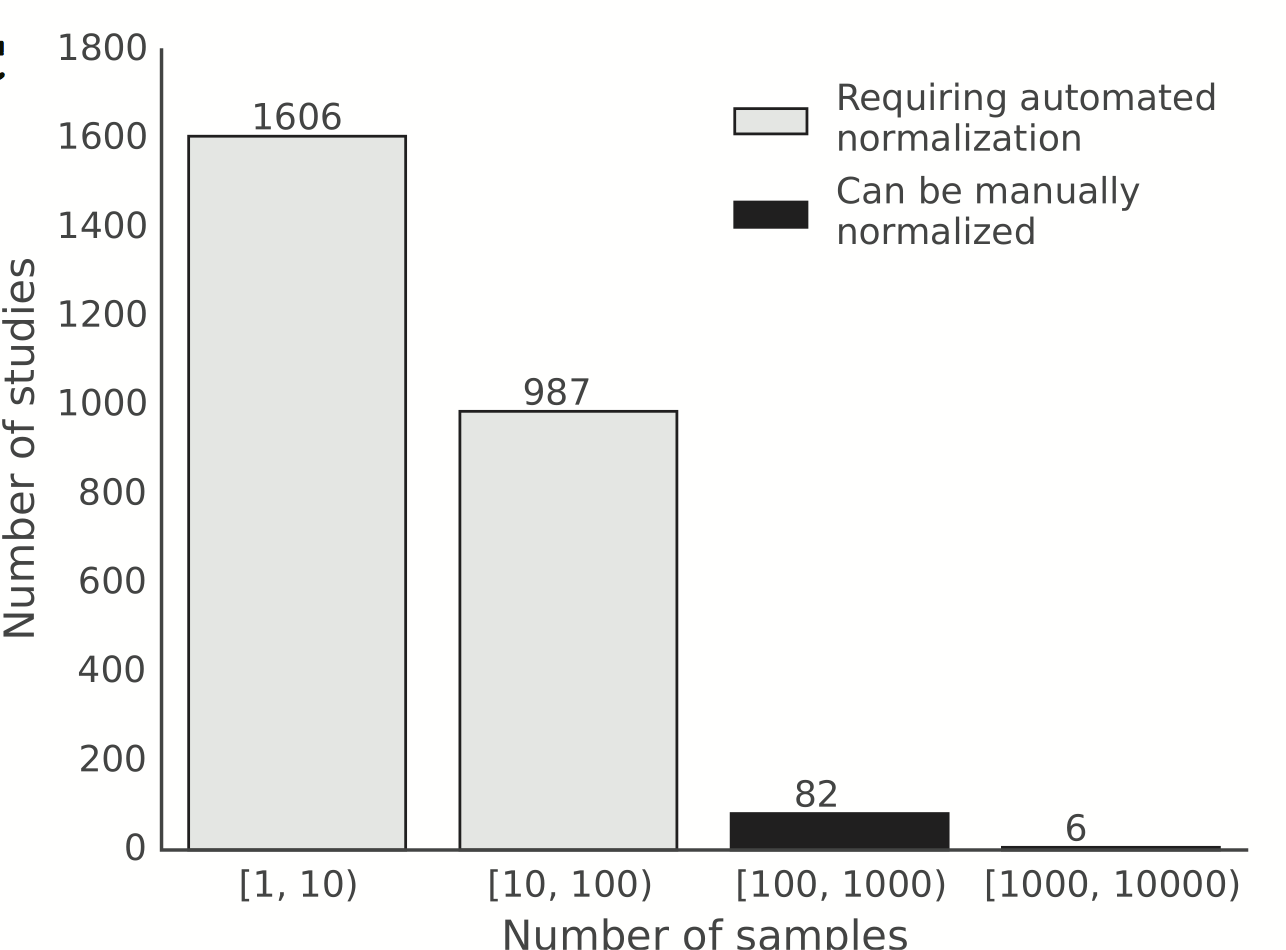
\includegraphics[scale=0.20]{figures/data_set_figure.png}}
\caption{\textbf{Dataset overview} Histogram of the number of samples per study for human RNA-seq experiments using the Illumina platform. We assert that the 88 studies each with at least 100 samples can be semi-manually normalized using study-specific methods.}
\label{fig:dataset}
\end{figure*}





\section{Methods}

Framing the ontology term mapping task as a multi-class classification problem in which each ontology term is a class, a machine learning approach might seem to be a natural choice.  However, such an approach would require a training set that includes multiple examples of samples that map to each ontology term.  Due to the large number of ontology terms, obtaining such a training set is unfeasible.  Thus, for the ontology term mapping and real-value property extraction tasks, we took an algorithmic approach.  In contrast, the sample-type classification task involves only a handful of possible classes and we can easily create, via manual annotation, a training set containing multiple samples from each class.  Thus, for this latter task, we used a statistical machine learning approach.

\subsection{Mapping samples to ontologies}

At the core of our method is a graph data structure for maintaining the provenance of each derived ontology term.  This graph, which we call a Text Reasoning Graph (TRG), provides a framework for maintaining the provenance of extracted ontology terms, and for writing rules and operations that can reason about which terms should be mapped versus which are merely mentioned.  Nodes in the TRG represent artifacts derived from the original metadata text. Such artifacts may be $n$-grams, inflectional variants, or synonyms.  Other nodes in the graph represent mapping targets such as ontology terms or real-value property tuples.  Edges between artifacts represent derivations from one artifact to another. An edge between an artifact and an ontology term represents a lexical match between the artifact and the ontology term.  

We implemented a computational pipeline that is composed of a series of stages that constructs the TRG.  To start, the pipeline accepts the raw key-value pairs and constructs an initial TRG. Then, each stage operates on the TRG by modifying its nodes and edges. Figure~\ref{fig:example_trg} depicts the subgraph of a final TRG that maps a key-value pair to a set of ontology terms.   By maintaining the provenance of each derived ontology term we can implement custom reasoning operations that more accurately determine which terms describe the sample.  Such reasoning operations utilize the graph structure to filter out ontology terms for which there is no relationship-type in $\mathcal{R}$ that describes the relationship between the sample and the ontology term.  

\begin{figure*}
\centerline{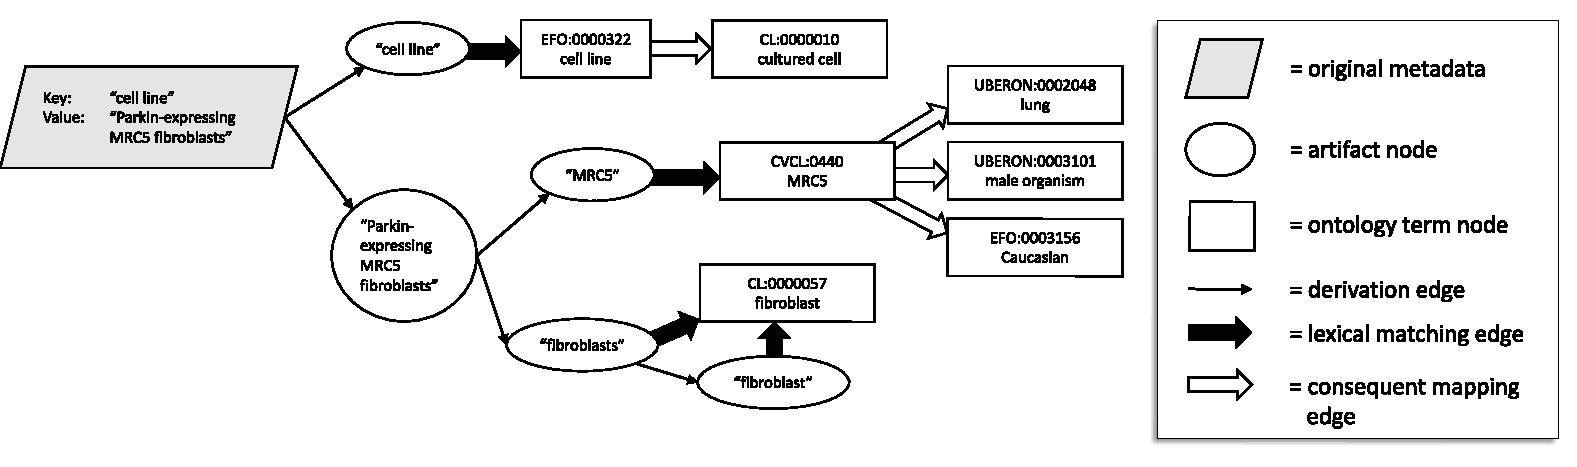
\includegraphics[width=13cm]{figures/example_TRG.pdf}}
\caption{\textbf{Example Text Reasoning Graph.} A subgraph of the TRG constructed from sample SRS1212219 illustrating the graph data structure that our pipeline maintains as it reasons about the sample.  This framework allows us to maintain the context of each artifact. For example, we map to the MRC5 cell line only because there is a mapping to the ``cell line'' ontology term in the graph emanating from the key.  We also note the terms for ``lung'', ``male organism'', and ``Caucasian'' were mapped to the MRC5 cell line from the ATCC cell bank data and are thus \textit{consequent mappings}.}
\label{fig:example_trg}
\end{figure*}

In the following sections we describe the most notable stages of the pipeline. Full details are provided in Section~\ref{sec:mapping_pipeline}.

\subsubsection{Filtering key-value pairs}

Before initializing the TRG, we filter key-value pairs from the metadata where either the key or value appears in a set of blacklisted keys and values.  This blacklist of keys contains those that describe a property that does not pertain to the biology of the sample, such as ``study name'' and ``biomaterial provider.''  The blacklist of values include those that negate the key, such as ``none'' or ``no.''  For example, the key-value pair \texttt{is tumor: no} is removed because the value \texttt{no} negates the property \texttt{is tumor}. 

\subsubsection{Artifact generation}

We define an artifact to be any string that is derived from a substring of the original metadata text.  Such artifacts include include $n$-grams, lower-cased words, and inflectional and spelling variants of words in the metadata.  An artifact node in the TRG represents a single artifact.  Several stages of the pipeline generate new artifact nodes from existing artifact nodes and draw edges from original to derived artifacts.   One such stage derives inflectional and spelling variants from existing artifacts using the National Library of Medicine's SPECIALIST lexicon (\citealp{Browne}).  For example, given an artifact node representing the pluralized noun ``fibroblasts'', this stage will create a node for the singular noun ``fibroblast'' and draw a directed edge from ``fibroblasts'' to ``fibroblast'' (Fig.~\ref{fig:example_trg}).

\subsubsection{Matching artifacts to ontologies}

We perform fuzzy string matching between all artifacts and  ontology terms to find all exact matches and minor misspellings (for misspelling criteria, see supplementary materials). For example, in Figure~\ref{fig:example_trg}, both the strings ``fibroblasts" and ``fibroblast" fuzzily match to the ontology term for ``fibroblast".

In general, fuzzy matching is computationally expensive.  To speed up this process, we pre-compute a  metric tree index (\citealp{Bartolini}) for all ontology term names and synonyms. The index allows us to filter for ontology term strings that are nearby the query string in edit space.  We then explicitly compute the edit distances to these nearby strings. 

\subsubsection{Graph reasoning}

Certain stages of the pipeline utilize the structure of the TRG.  We refer to such steps as ``reasoning'' steps.  For example, we remove extraneous mappings to cell line terms by searching the graph emanating from the key for a lexical match to ontology terms such as ``cell line'' and ``cell type.''  If such a match is \textit{not} found, we search the graph emanating from the value for artifacts that have a lexical match to a cell line ontology term and remove all such ontology term nodes.  This process is important for removing false positives due to the fact that names of cell lines are often similar to gene names and acronyms. For example, ``Myelodysplastic Syndromes'' is often shortened to ``MDS.'' MDS also happens to be a cell line in the Cellosaurus. Other examples of stages that utilize the graph structure are described in the supplementary materials.

\subsubsection{Inferring consequent terms}

Certain stages of the pipeline attempt to map the sample to terms that are not explicitly mentioned in the raw metadata text describing the sample.  We refer to such mapped terms as \textit{consequent terms}.  We map to consequent terms by consulting external knowledge bases.  The pipeline uses two external knowledge bases: a cell line database and a rules database.

First, we created a database of mappings between cell lines and ontology terms.  We obtained this data by scraping from the ATCC website (\href{https://www.atcc.org}{https://www.atcc.org}). We scraped cell line metadata for all cell lines that are present in the Cellosaurus.  To construct mappings between cell lines and ontology terms, we ran a variant of our pipeline on the scraped cell line data. Our pipeline uses this database as follows: our pipeline will draw edges between mapped cell line ontology term nodes and the ontology terms that describe the biology of the cell line.   For example, in Figure~\ref{fig:example_trg}, the ontology term for the MRC5 cell line has an edge to ``lung", ``male", and ``Caucasian" because this cell line was derived from lung tissue of a Caucasian male aborted fetus (\citealp{Jacobs}).

Second, we created a small rules database that dictates how certain ontology terms logically imply other ontology terms.  For example, in Figure~\ref{fig:example_trg} the term ``cell line" has an edge to the term ``cultured cell" because all cell lines are grown in a culture.  

\subsubsection{Maximal phrase-length mapping}

It is a common occurrence for disease ontology terms to include anatomical entities in their name. For example, ``breast cancer'' includes ``breast'' as a substring. As previously discussed, under our framework, it would be incorrect to map ``breast'' to a sample solely based on a mention of ``breast cancer'' in its metadata because ``breast'' localizes the cancer, but does not localize the origin of the sample.  Whereas it is entirely possible that such a sample was indeed derived from breast tissue, without additional information we cannot eliminate the possibility that the sample originated from some other tissue, such as from a malignant site.  In this example, we maintain a conservative approach and avoid mapping to ``breast.''  We implement this process by having each artifact node keep track of the original character indices in the metadata from which it was derived. After mapping all artifacts to the ontologies, we remove all ontology terms that were lexically matched with an artifact node that is subsumed by another artifact node that matches with an ontology term.  

\subsubsection{Linking ontologies}

The domain covered by the EFO overlaps with many of the other ontologies because it includes cell types, anatomical entities, diseases, and cell lines.  In many cases, the EFO is inconsistent with other ontologies in how it draws edges between terms.  For example, the term ``lung adenocarcinoma'' and ``adenocarcinoma'' are present in both the Disease Ontology and the EFO; however ``adenocarcinoma'' is a parent of ``lung adenocarcinoma'' in the Disease Ontology but not in the EFO.  These inconsistencies pose a problem when we apply our maximal phrase-length mapping process.   For example, when a sample maps to ``lung adenocarcinoma'' and ``adenocarcinoma'', we remove ``adenocarcinoma'' because it is a substring of ``lung adenocarcinoma.''  This is valid for the Disease Ontology because the term for ``adenocarcinoma'' is implied by ``lung adenocarcinoma'' by its position in the ontology.  However, this results in a false negative for the EFO version of this term.  

To counteract this problem, we link EFO terms to terms in the other ontologies.  Two terms are linked when they share the same term-name or exact-synonym.  Then, when an artifact maps to a term, we traverse the term's ancestors and map to any terms that are linked to those ancestors.   In the case of ``lung adenocarcinoma'', we would traverse the ancestors of this term in the Disease Ontology and map to the EFO's ``adenocarcinoma'' because it is linked to the Disease Ontology version of this term. Figure~\ref{fig:linked} illustrates this process. 

\begin{figure}[htbp]
\centering
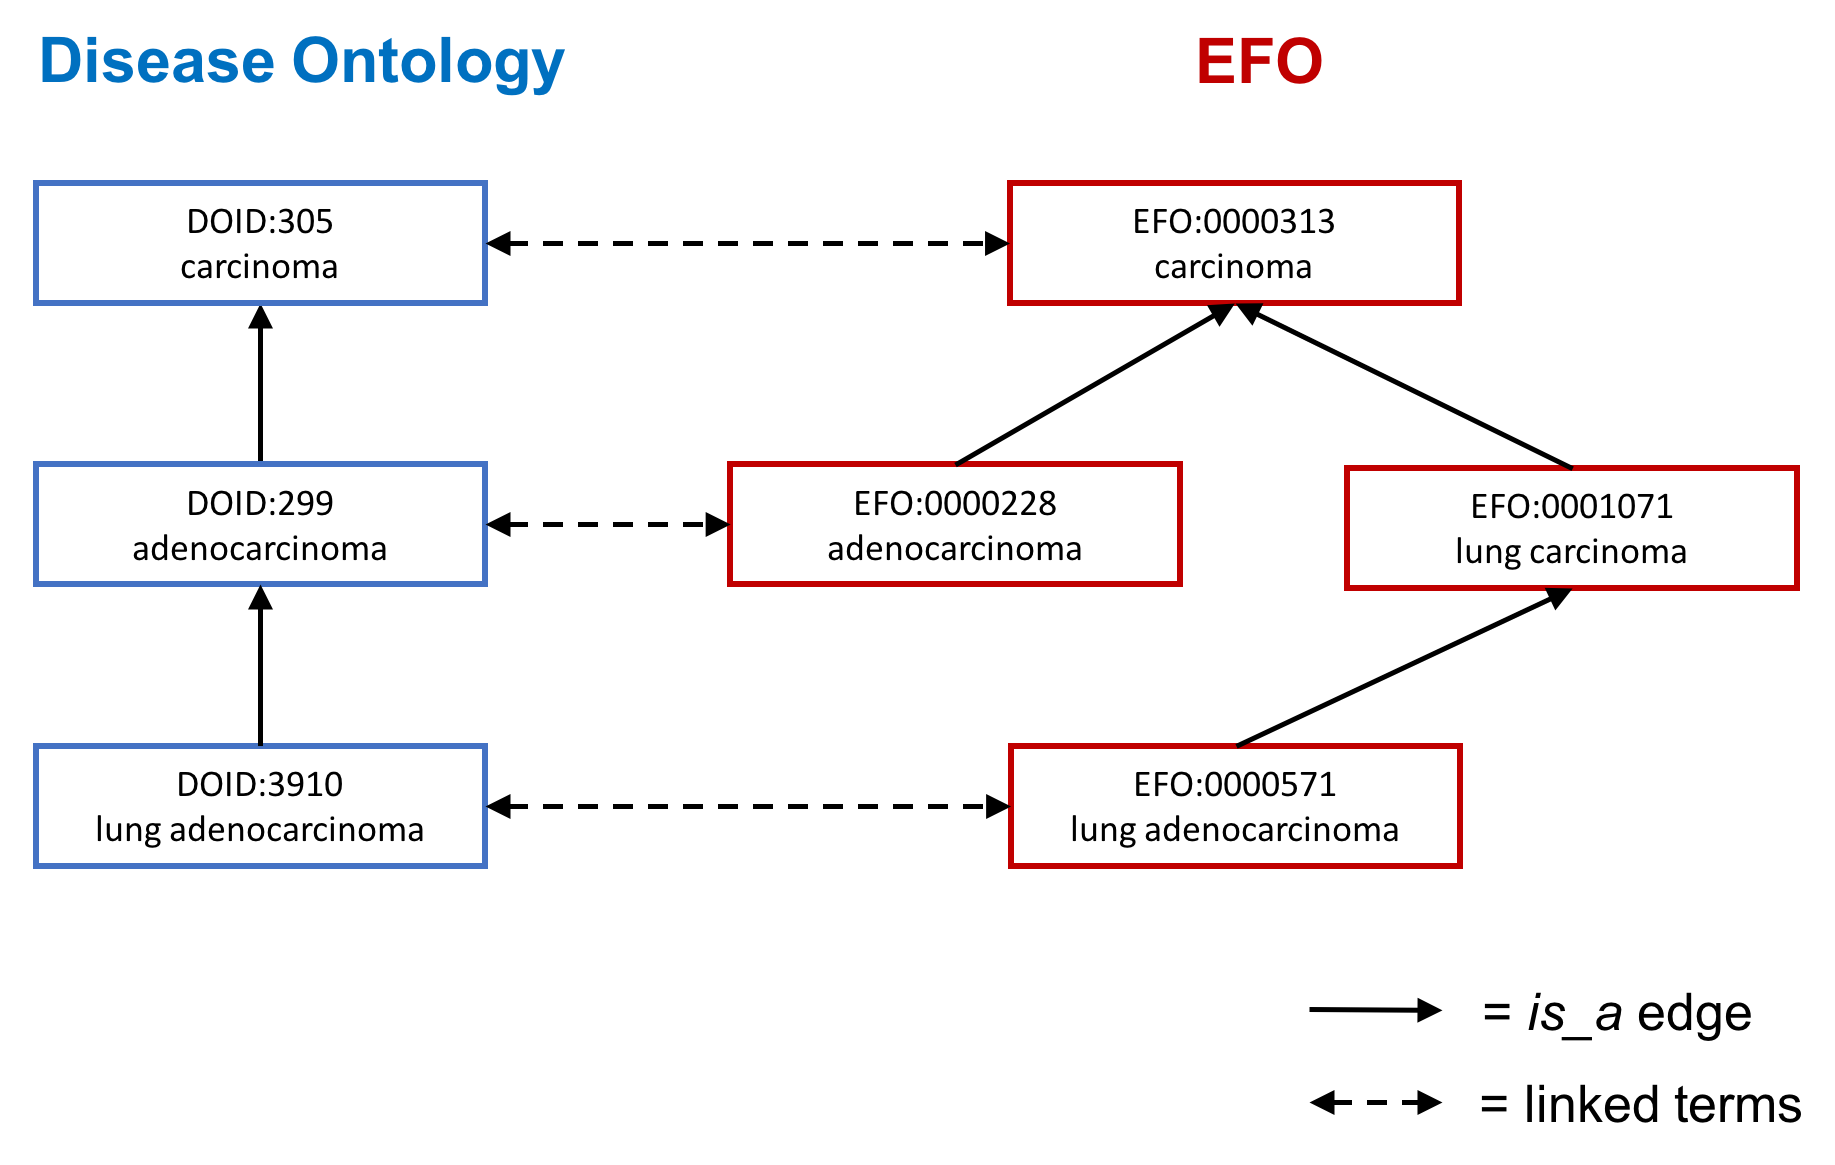
\includegraphics[scale=0.35]{figures/linked_ontologies.png} 
\caption{\textbf{Linking ontologies.} An example of linked terms between the Disease Ontology and the EFO. If a sample maps to ``lung adenocarcinoma'' in the Disease Ontology, we follow all ancestors and also map to linked terms of those ancestors. In this case, the EFO's ``adenocarcinoma'' term will also be mapped.}
\label{fig:linked}
\end{figure}

\subsection{Extracting real-value properties}
We maintain a list of ontology terms that define real-value properties. Currently, we use 6 terms: ``age'', ``passage number'', ``timepoint'', ``age at diagnosis", ``body mass index", and ``age at death."  Future work will entail expanding this list.  To extract a real-value property from a key-value pair, we search the graph emanating from the key for a match to a property ontology term.  If such a property is found, we search the graph emanating from the value for an artifact representing a numerical value and a unit ontology term node (e.g., ``46'' and ``year'').  From this process, we extract the triple (property, value, unit). For example, given the key-value pair \texttt{age: 46 years old}, we extract (``age'', 46, ``year'').

\subsection{Predicting sample-type category}\label{prediction_sample_type}

We classify samples by sample-type using a supervised machine learning approach.  This stands in contrast to the non-statistical approach used in the aforementioned ontology term mapping task. We trained a one-vs.-rest ensemble of logistic regression, binary classifiers  
%That is, each classifier learns a model of the form
%$$p(y = 1 | \bold{x}) := \left[1+\exp(\boldsymbol{\beta}^\top\bold{x})\right]^{-1}$$
%where $y=1$ indicates the sample belongs to the class, $\boldsymbol{\beta}$ are coefficients assigned to each feature, and $\bold{x}$ is the feature vector. 
where each classifier was trained using L1 regularization.  For each sample, the classifier accepts as input both the raw key-value metadata as well as the ontology terms that were mapped by our aforementioned pipeline.  The classifier then outputs the sample's predicted sample-type.

We consider two types of features for representing each sample: $n$-gram features and ontology term features.  For $n$-gram features, we consider all uni-grams and bi-grams appearing in the training samples' raw metadata.  For ontology term features, we consider the set of all ontology terms that were mapped to the training samples by our automated ontology-term mapping pipeline.  We performed a feature selection process (for details, see supplementary materials) that involved using mutual information to select features that are indicative of at least one of the target sample-types. 

When making a prediction on a sample $x$, each logistic regression binary classifier $c_j$ in the ensemble computes its estimate of the conditional probability $c_j(x) := p(y = j | x)$, which can be interpreted as the confidence that classifier $c_j$ believes that $x$ is of type $j$.  Using these probabilities, we designed a decision procedure that uses our domain knowledge for determining the sample-type.  Specifically, we limit the possible sample-types based on the ontology terms mapped to the sample. For example, if ``stem cell'' was mapped to the sample, we limit the possible predictions to \texttt{stem cells}, \texttt{induced pluripotent stem cell line}, and \texttt{in vitro differentiated cells}.  We found that injecting such domain knowledge into the process boosted performance in cross-validation experiments. See Section~\ref{sec:sample_pred} for details.  Although theoretically, the learning algorithm should learn these facts itself, there is likely not enough training examples for the algorithm to learn such patterns.

We randomly sampled and manually annotated \SampleTypeTrainingSetSize{} samples based on their metadata. We determined each sample's sample-type by consulting the sample's study, publication, and other external resources that describe the experimental procedure used to obtain the sample.  Four of these samples did not adequately fit into any sample-type category and thus were excluded from training. Since samples that belong to the same study are likely described similarly, one potential pitfall in the learning process is that if training samples are drawn uniformly and at random from all samples, the learner will be biased towards features that correlate with how larger studies describe their samples rather than features that correlate with sample-type.  To avoid this issue, we ensured that no two samples in the training set came from the same study. 




\section{Results}

\subsection{Evaluation of ontology mappings}\label{sec:eval_onto_mappings}

In order to create a test set for evaluation of our pipeline, we manually normalized metadata for \TestSetSize{} samples from the SRA where each sample belongs to a unique study. This test set was obtained by randomly sampling from entries that were recently added to the archive and had not been considered during the development of our computational pipeline. Thus, performance on this subset of data provides an unbiased estimate of its ability to generalize to unseen samples.  We note that these \TestSetSize{} samples are disjoint from the \SampleTypeTrainingSetSize{} samples described in section~\ref{prediction_sample_type} that were used to train the sample-type classifier. 

\begin{figure*}[!tpb]
\centerline{\includegraphics[width=13cm]{figures/results_fig.eps}}
\caption{\textbf{Ontology term mapping results.} (A) A schematic of an ontology subgraph demonstrating our calculation of recall, specific terms recall, error rate, and specific terms error rate.  (B) Performance of our pipeline in mapping explicit ontology terms versus BioPortal's Annotator, ZOOMA, and SORTA.  We ran SORTA using the three confidence thresholds of 1.0, 0.5, and 0.0. We also ran ZOOMA using the three confidence thresholds of high, good, and low.  We measured recall, error rate, specific terms recall, and specific terms error rate for all programs across all ontologies with the exceptions that ZOOMA only maps to three of the ontologies and only MetaSRA and SORTA map to the Cellosaurus. (C) The error rate, specific terms error rate, average retrieved terms per sample, and average specific retrieved terms per sample across all ontologies when considering only consequently mapped terms.  No terms from the Cellosaurus were consequently mapped and thus this ontology is omitted.  (D) Recall, error rate, specific terms recall, and specific terms error rate for versions of our pipeline in which certain stages are disabled.  The data points labelled ``none'' refer to the complete pipeline in which no stage is disabled.}\label{fig:results}
\end{figure*}

We first evaluated our pipeline's ability to map samples to explicitly mapped ontology terms using the following metrics: recall, error rate, specific terms recall, and specific terms error rate.  Given a sample, let $T$ be the set of all ontology terms to which the sample maps including terms ancestral to those explicitly mentioned.  Let $T'$ be the most specific terms in $T$.  That is $T' := \{t \in T : \text{no child of $t$ is in T}\}$.  Let $P$ be the set of predicted terms to which the sample maps.  Let $P'$ be the most specific terms in $P$. That is $P' := \{p \in P : \text{no child of $p$ is in P}\}$.  We define our metrics as follows: 
\begin{align*}
\text{recall} &:= \frac{|T \cap P|}{|T|}&
\text{specific terms recall} &:= \frac{|T' \cap P|}{|T'|}
\\
\text{error rate} &:=  \frac{|P \setminus T|}{|P|}&
\text{specific terms error rate} &:=  \frac{|P' \setminus T|}{|P'|}
\end{align*}
 We use these four metrics instead of traditional precision and recall because precision and recall are affected by the structure of the ontology.  This is due to the fact that the act of retrieving an ontology term implicitly retrieves all of its ancestral terms in the ontology's directed acyclic graph.  Thus, retrieving a term with a high number of ancestral terms will lead to exaggerated metrics.  The specific terms error rate corrects for this by describing the fraction of the most specific predicted terms that incorrectly describe the sample.  We note that the error rate is simply $1 - \text{precision}$.  The metrics are demonstrated in Figure~\ref{fig:results}A. 

With these metrics, we compared our pipeline to the BioPortal Annotator, SORTA, and ZOOMA across all ontologies (Fig.~\ref{fig:results}B).  Compared to these methods, our pipeline has a low error rate while maintaining a competitive recall.  For example, although the ZOOMA pipeline scores a slightly lower error rate on the Disease Ontology, Cell Ontology, and Uberon than our pipeline, this comes at the cost of a much lower recall. Similarly, although the SORTA tool scores a slightly higher specific terms recall on the Disease Ontology and Cell Ontology than our pipeline, this comes at the cost of a much higher error rate.  Lastly, we note that our pipeline scores a higher recall and lower error rate across all ontologies when compared to the BioPortal Annotator.  

We then evaluated the pipeline's ability to map consequent terms. Recall is an inappropriate metric for evaluating our ability to map consequent terms  due to the fact that the set of consequent terms is undefined.  By our definition, a consequent term is any term that the sample can be mapped to based on expert or external knowledge.  Thus, depending on the expert or external knowledge base, the set of consequent terms may change.  Furthermore, an expert may use an exceedingly large number of ontology terms to describe the sample depending on what she knows about the sample and experiment. For these reasons, we look at the total average number of consequent terms that we map to each sample.  This metric describes the amount of extra information that is provided when considering external knowledge.  We further looked at the average number of most specific mapped consequent terms.   Figure~\ref{fig:results}C displays these metrics across the ontologies.

Lastly, we evaluate the performance impact of each of our pipeline's stages, we ran our pipeline on our test set with certain individual stages disabled.  Figure~\ref{fig:results}D shows the performance impact when removing stages for filtering key-value pairs, linking ontologies, filtering sub-phrase matches,  and generating spelling and inflectional variants. As expected, the results of these tests indicate a general trade off between recall and error rate.  Certain stages may decrease recall, but pose the benefit of decreasing the error rate.  Furthermore, a given stage may be more effective for mapping terms in some ontologies rather than others.

Finally, we evaluated performance on the top 10 most commonly mapped terms.  For this analysis, we count a term as being mapped from a sample if that term is a most-specifically-mapped term for that sample.  That is, no children of the term were mapped from the sample.  For each term in the top 10 most commonly mapped terms, we sampled 100 samples at random from the entire set of samples in the MetaSRA.  For this analysis, we allowed multiple samples from the same study.  We then evaluate the precision for the target term over these 100 samples. The results are displayed in Table \ref{table:top_terms}.  These statistics provide an unbiased estimate of the precision for each term over the entire set of samples in the MetaSRA.  

    \begin{table}[h!]
    \begin{center}
    \begin{tabular}{ |c|c|c| } 
    \hline
    Term & Name & Precision \\ \hline
    CL:0000010 & cultured cell & 0.98 \\
    UBERON:0003100 & female organism & 1.00 \\
    UBERON:0003101 & male organism & 1.00 \\
    UBERON:0000955 & brain & 0.99 \\
    EFO:0000727 & treatment & 0.90 \\
    UBERON:0000178 & blood & 0.86 \\
    EFO:0003156 & Caucasian & 1.00 \\
    EFO:0000322 & cell line & 1.00 \\
    EFO:0001272 & adult & 1.00 \\
    UBERON:0007023 & adult organism & 1.00 \\
    \hline
    \end{tabular}
    \end{center}
    \caption{\textbf{Precision of the most commonly mapped ontology terms.}}
    \label{table:top_terms}
    \end{table}


\subsection{Evaluating extraction of real-value properties}

Of the \TestSetSize{} samples in our test set, \TestSetRealValSize{} described real-value properties.  We evaluated our performance in retrieving real-value property tuples in terms of precision and recall. A predicted real-value property was called a true positive if the property type, value, and unit all matched the ground truth.  On the \TestSetRealValSize{} samples, we report precision of \RealValPrecision{} and recall of \RealValRecall{}. We note that the high precision our method achieves is due to the heavy constraints we place on calling a real-value property, which also result in relatively low recall.

\subsection{Evaluating sample-type predictions}

\begin{figure*}[!tpb]
\centerline{\includegraphics[width=13cm]{figures/sample_type_prediction_results.eps}}
\caption{\textbf{Sample-type prediction results.} (A) Row-normalized confusion matrix for sample-type category prediction accuracy on the initial test data set. Element $i,j$ is the fraction of samples in category $i$ that were labelled as category $j$ by the classifier. The diagonal elements are category-specific recall values.  The number of samples in each category are shown above the matrix. (B) Transpose of the column-normalized confusion matrix for sample-type category on the enriched test data set.  Element $i, j$ represents the fraction of samples labelled as category $i$ that are truly category $j$. The diagonal elements are category-specific precision values. The number of samples predicted to be in each category are shown above the matrix.   (C) Calibration of the model.  The estimated probability of the model (average of confidence values in each bin) is plotted against the empirical probability that the model is correct (accuracy of predictions in each bin). The straight blue-line plots a well-calibrated model. Error bars are drawn according to a bootstrap sampling approach (\citealp{Brocker}). Points are omitted for bins that contain no predictions. This plot was created from the initial data set of \TestSetSize{} samples.}
\label{fig:sample_type}
\end{figure*}

To evaluate our ability to predict each sample's sample-type, we evaluated the algorithm's performance on two held-out test sets. The first test data set was created by manually annotating the sample-types for the \TestSetSize{} samples that were used for evaluating our ontology term mapping procedure.  As noted previously, no two samples in this data set belong to the same study.   We annotated all samples for which the origin of the sample was explained in an external resource such as a scientific publication. In total, this came to \NonEnrichedSampleTypeTestSetSize{} samples.  The distribution of sample-types in our test set is illustrated in the bar graph above the matrix in Figure~\ref{fig:sample_type}A.

Our trained classifier achieved an accuracy of \SampleTypeOverallAccuracy{} over these samples.  The confusion between categories is plotted in Figure~\ref{fig:sample_type}A.  In general, the classifier does well in determining the cell line samples and tissue samples.  Close inspection of the classifier's errors revealed that most were due to samples with descriptions of poor quality.  Such samples are difficult to categorize, even as a human, without consulting the scientific publication in which the sample is described. Correctly classifying these samples will require utilizing external descriptions of the samples. 

Because this test set of \TestSetSize{} samples is impoverished for some sample-types, we enriched it by sampling additional samples from each predicted sample-type category, continuing to ensure that no two samples belonged to the same study.  We sought at least 100 samples that were predicted to fall in each category; however for \texttt{primary cells}, \texttt{stem cells}, and \texttt{induced pluripotent stem cell line} samples, we were unable to achieve this threshold given our criteria. This resulted in a test data set consisting of \EnrichedSampleTypeTestSetSize{} samples.  We used this enriched test data set to better estimate the category-specific precision of our classifier (Fig.~\ref{fig:sample_type}C).  Since the sampling procedure used for the enriched test data set was biased by the predicted sample-type of each sample, it could not be used for an unbiased estimate of recall or overall accuracy.

MetaSRA includes the classifier's confidence of each prediction. To evaluate the quality of these confidence scores, we assessed the calibration of the classifier.  A classifier is well calibrated if for any instance $x$ with true label $y$, it holds that $\hat{p} = p(\hat{y} = y)$ where $\hat{y}$ is the classifier's predicted class label of $x$ and $\hat{p}$ is its confidence. To assess calibration, we grouped the predictions  into bins according to their confidence scores and compute the empirical accuracy of predictions in each bin (Fig.~\ref{fig:sample_type}B).  We found the classifier to be well calibrated, and thus that its confidence scores may be of use in filtering predictions to a achieve a target accuracy level.

We note that the test data set was small compared to the training data set. To provide an estimate of the performance of the classifier on a larger data set, we ran the algorithm using leave-one-out cross validation on the training set. The algorithm achieved 0.845 accuracy on this data set.  Figure~\ref{fig:train_set}A shows the row-normalized confusion matrix and Figure~\ref{fig:train_set}B shows the calibration of the model.

\begin{figure}[htbp]
\centering
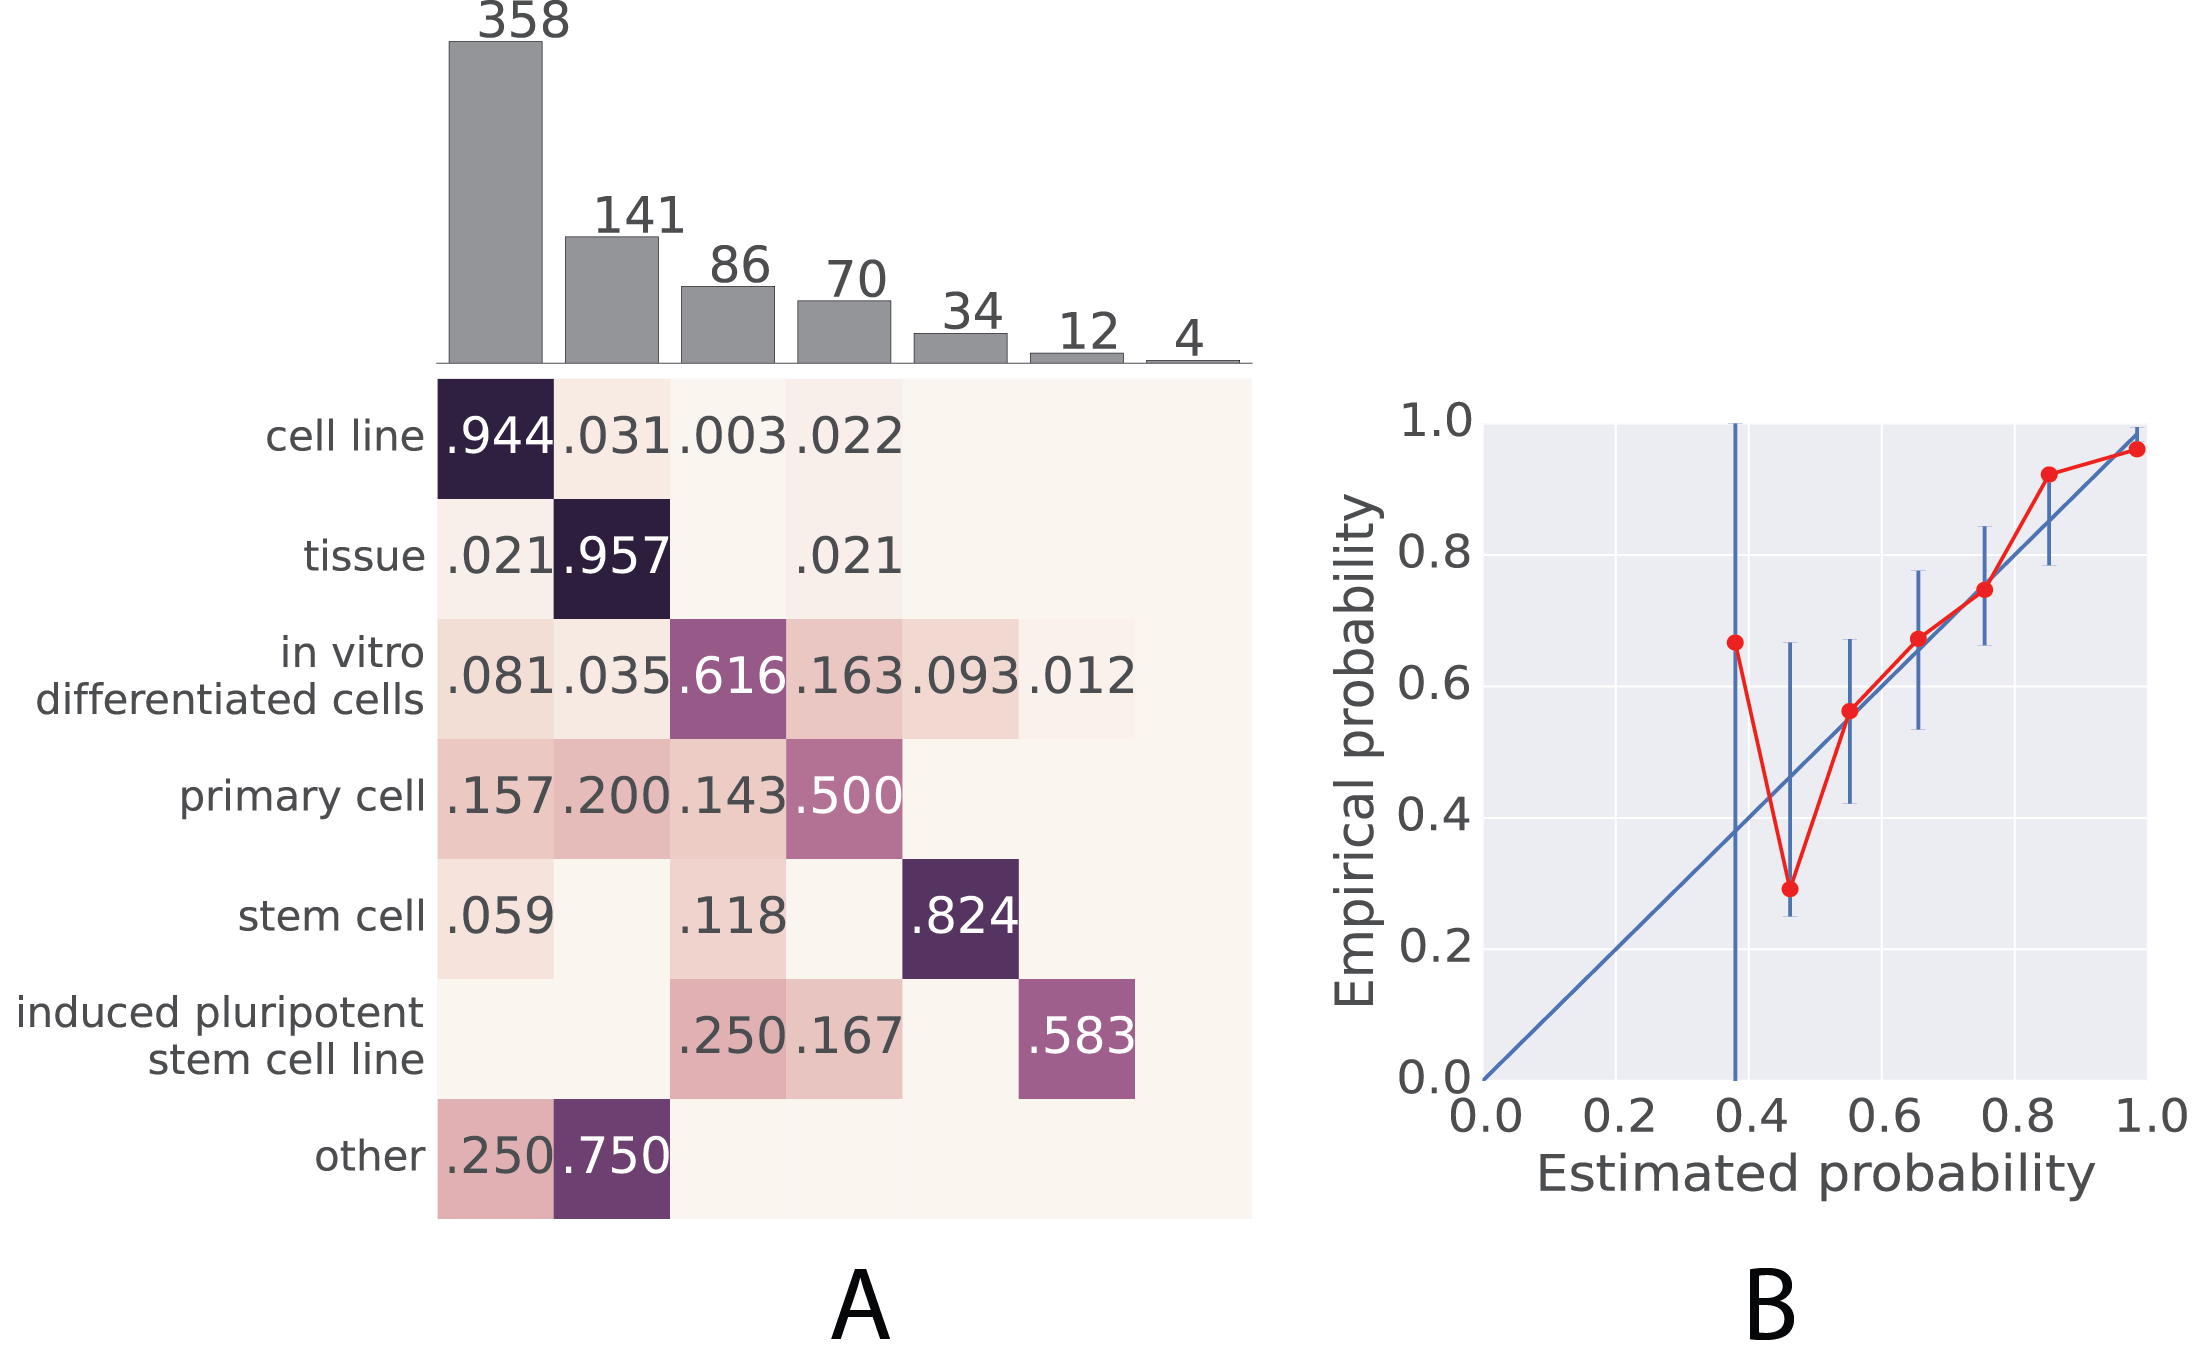
\includegraphics[width=13cm]{figures/sample_type_training_set.png} 
\caption{\textbf{Sample-type prediction results on the training set.} (A) The confusion matrix of the algorithm on the training set evaluated using leave-one-out cross validation. The bar graph above the matrix displays the distribution of classes within the training set. (B) Plotting the calibration of the classifier.}
\label{fig:train_set}
\end{figure}


\subsection{Summarizing the MetaSRA}\label{sec:sum_metasra}

We summarized the contents of the MetaSRA run on all samples, including those that belong to the ``large'' ($\geq 100$ samples) studies.  First, we explored the distribution of the number of samples mapped to each ontology term (Fig.~\ref{fig:metasra_summary}A).  Most terms from each ontology map to fewer than 100 samples, whereas a few terms map to upwards of 10,000 samples.  Second, we looked at the fraction of samples that were mapped to terms within each ontology (Fig.~\ref{fig:metasra_summary}B).  The fraction of samples mapping to each ontology differed markedly between samples of different predicted sample type, which provides some insight into how the sample-type classifier makes its decisions.  For example, tissue samples tend to be described by an anatomical term in the Uberon ontology and not described by a specific cell type in the Cell Ontology. 
Lastly, we identified the most common ontology terms (Fig.~\ref{fig:metasra_summary}C) 
%and real value properties (Table~\ref{tab:real_val_props})
in the MetaSRA.  In general, the error rate for the most common ontology terms was quite low.

\begin{figure*}[!tpb]
\centerline{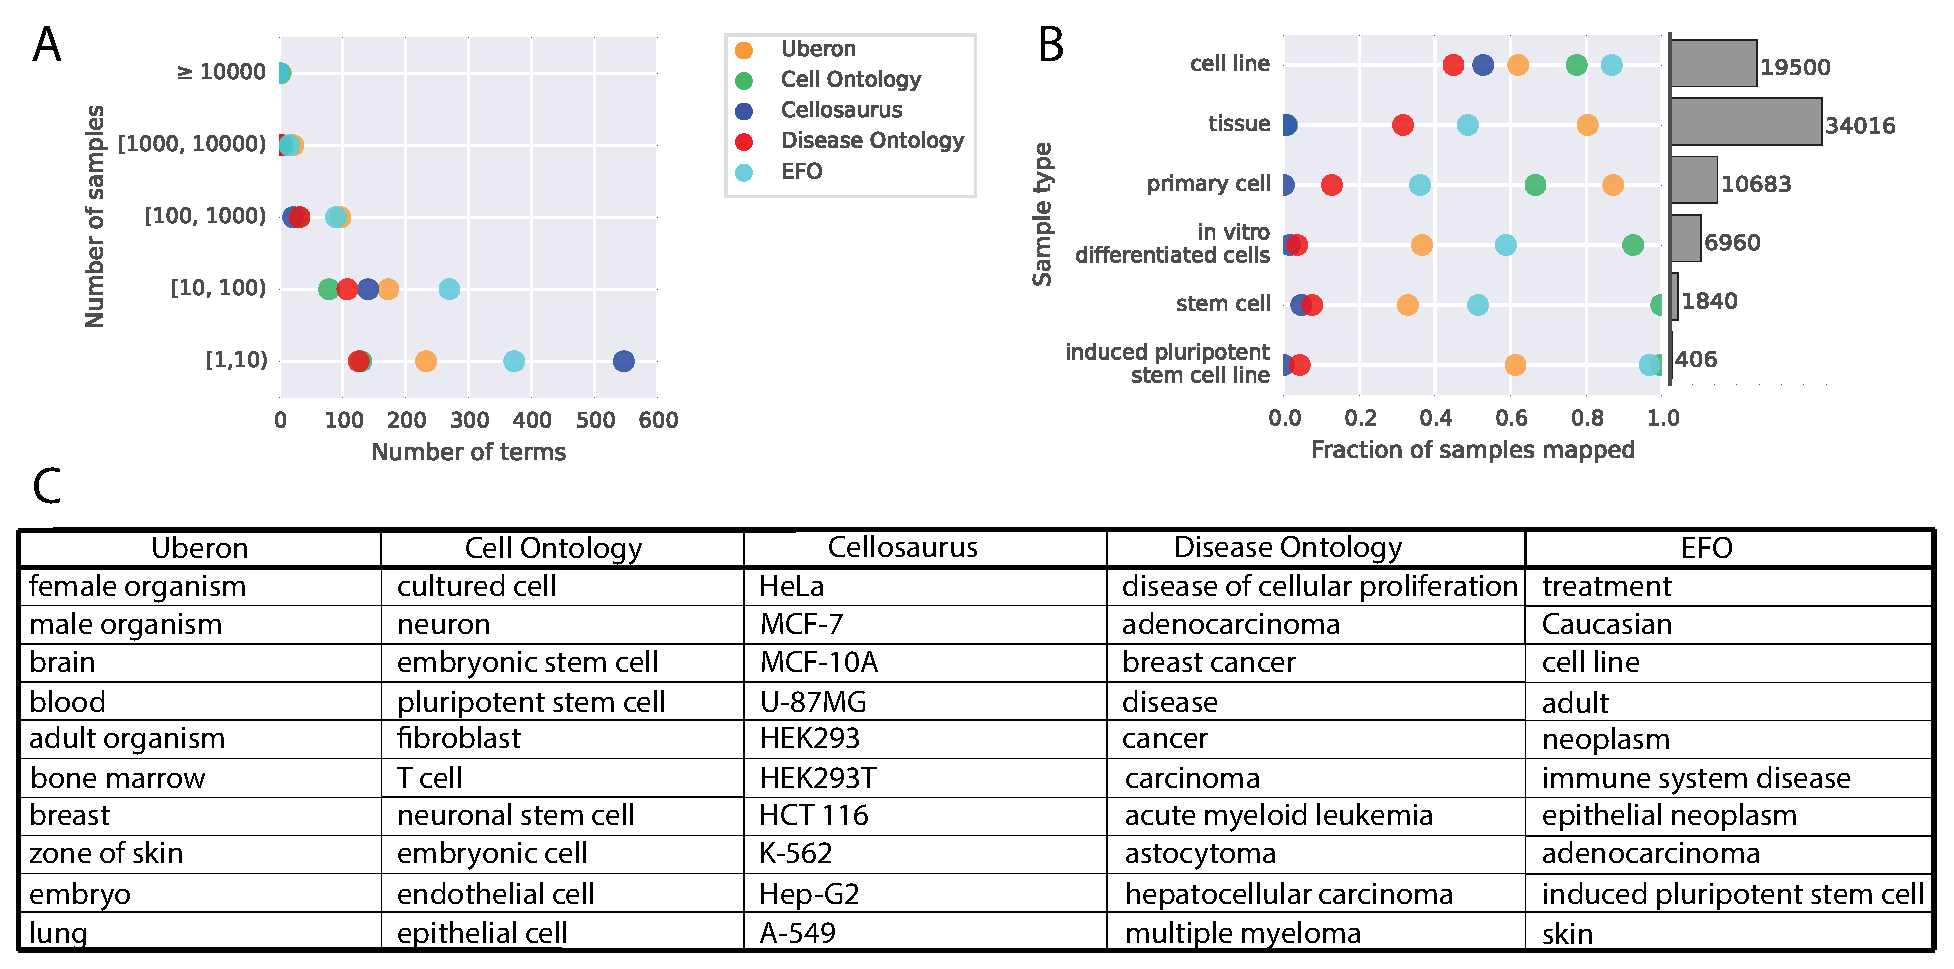
\includegraphics[width=13cm]{figures/metasra_summary.eps}}
\caption{\textbf{Summary of the MetaSRA.} (A) The number of terms from each ontology that map to a given range of number of samples.  Only the most-specifically mapped terms for each sample are considered. (B) Fraction of samples of each predicted sample-type that map to each ontology. The bar plot to the right of the strip-plot shows the number of each predicted sample-type. (C) The most commonly mapped terms for each ontology. Only the most-specifically mapped terms for each sample are considered.}
\label{fig:metasra_summary}
\end{figure*}

%\begin{table}[!th]
%\processtable{The number of samples in the MetaSRA that are annotated with each real-value property. Overall, \PercentageMetaSRARealVal{}\% of samples were mapped to a real-value property.\label{tab:real_val_props}} {\begin{tabular}{@{}lll@{}}\toprule
%Property & Number of samples & Percentage of samples \\ \midrule
%        age & 12416 & 16.9 \\
%passage number & 3307 & 4.5 \\
%timepoint & 831 & 1.1 \\
%age at diagnosis & 645 & 0.9 \\
%body mass index & 200 & 0.3 \\
%age at death & 98 & 0.1 \\
%\botrule
%\end{tabular}}{}
%\end{table}





























